\documentclass[fr,license=none]{../../../../../../eplexam}
\usepackage{multirow}
\usepackage{../../../../../../eplunits}
\usepackage{../../../../../../eplcommon}
\usepackage{enumitem}
\usepackage{tikz}
\usetikzlibrary{arrows.meta}

\hypertitle{Mod\`eles et m\'ethodes d'optimisation}{4}{INMA}{1702}{2011}{Juin}{Majeure}
{Gilles Peiffer}
{Vincent Blondel et François Glineur}

\newcommand{\libre}{\ensuremath{\textnormal{ libre}}}
\newcommand{\redcost}{\tilde{c}} % Coût réduits
\newcommand{\xopt}{\ensuremath{x^*}}
\newcommand{\zopt}{\ensuremath{z^*}}
\newcommand{\adset}{\mathcal{D}}
\newcommand{\eqset}{\mathcal{E}}
\newcommand{\inset}{\mathcal{I}}
\newcommand{\acset}{\mathcal{A}}
\newcommand{\lagr}{\mathcal{L}}
\newcommand{\dset}{\mathcal{C}}
\newcommand{\polye}{\mathcal{P}}
\newcommand{\sign}{\mathrm{sign}}
\newcommand{\rpm}{\sbox0{$1$}\sbox2{$\scriptstyle\pm$}
  \raise\dimexpr(\ht0-\ht2)/2\relax\box2 }
\newcommand*\mean[1]{\bar{#1}}
\newcommand{\irow}[1]{% inline row vector
  \begin{smallmatrix}(#1)\end{smallmatrix}%
}
\newcommand*\circled[1]{\tikz[baseline=(char.base)]{
            \node[shape=circle,draw,inner sep=2pt] (char) {#1};}}

\tikzset{dotnode/.style={fill=white,circle}}
\tikzset{noedge/.style={draw=white,very thick}}


\section{Réorganisation générale !}

On note $C_i$ chacune des $N = 589$ communes de Belgique.
Pour chaque couple de communes $(C_i, C_j)$, on connaît la distance
$d_{ij}$ qui les sépare, ainsi que le nombre de personnes $f_{ij}$
habitant à $C_i$ et travaillant à $C_j$.

\begin{enumerate}[label=(\alph*)]
     \item Supposez que chaque personne puisse décider d’aller habiter dans la
     commune de son choix, sous la contrainte que les populations actives
     totales de chaque commune ne peuvent être modifiées (le nombre de
     logements dans chaque commune est constant !).
     Dans ces conditions, proposez un modèle d’optimisation
     \textit{linéaire en nombres entiers} qui permettrait de minimiser la
     distance totale parcourue par la population active pour se rendre sur son
     lieu de travail.

     \textit{Note} : comme il n’est pas réaliste de considérer un modèle
     introduisant une ou plusieurs variables par personne, vous choisirez pour
     variables les nombres $x_{ij}$ de personnes travaillant à $C_j$ et
     habitant à $C_i$ après la réorganisation.

     \item À priori, votre modèle est en nombres entiers. Est-ce que la
     relaxation continue de votre problème fournit toujours une solution
     entière ? Si oui : prouvez-le ; si non : fournissez un contre-exemple avec
     une petite valeur de $N$.

     \item  Il n’est probablement pas réaliste de supposer que la totalité de
     la population active est potentiellement prête à déménager. Formulez de
     façon linéaire chacune des deux contraintes additionnelles suivantes :
     \begin{enumerate}[label=(\roman*)]
          \item \label{i} Seule une proportion $0 \le p \le 1$ de la
          population active \textit{totale} est disposée à déménager.
          \item \label{ii} Dans chaque \textit{ville}, seule une proportion
          $0 \le v \le 1$ de la population active de la ville est disposée à
          déménager.
     \end{enumerate}
     Classez ensuite (\textit{en justifiant}) les valeurs optimales (distances
     totales parcourues) des cinq problèmes suivants : problème original,
     problème avec contrainte \ref{i} et $p = 0.5$ puis $p = 0.75$, problème
     avec contrainte \ref{ii} et $v = 0.25$ puis $v = 0.5$.
\end{enumerate}

\begin{solution}
     \textit{Note} : cette solution s'inspire grandement de la solution
     proposée par les enseignants.\\


     Commençons par définir deux variables concernant la population.

     \begin{align*}
          \textnormal{Soit } P_i &= \sum_{j = 1}^{N} f_{ij}
          \textnormal{ la population totale habitant dans la ville } C_i \\
          T_j &= \sum_{i = 1}^{N} f_{ij}
          \textnormal{ la population totale travaillant dans la ville } C_j.
     \end{align*}

     \begin{enumerate}[label=(\alph*)]
          \item Voici la formulation du problème sous forme d'un problème
          d'optimisation linéaire en nombres entiers.

          \begin{equation*}
          \setlength\arraycolsep{1.5pt}
            \begin{array}{c@{\quad} r c r@{\qquad} c}
              \min\limits_{\mathclap{\substack{x_{ij} \in \N \\ 1 \le i,j \le N}}} & \sum\limits_{i =
               1}^{N} \sum\limits_{j = 1}^{N} d_{ij} f_{ij} & & & \\
              \mathrm{s.t.} & \sum\limits_{j = 1}^{N} x_{ij} & = & P_i & \forall i \in \{1, 2, \dots, N\} \\
              & \sum\limits_{i = 1}^{N} x_{ij} & = & T_j & \forall j \in \{1, 2, \dots, N\}.
            \end{array}
          \end{equation*}

          La première contrainte indique que la population d'une ville est
          constante, la seconde que le nombre de personnes travaillant dans une
          ville est constant.

          Il s'agit en réalité d'un problème de transport.

          \item Un problème de transport peut être modélisé par un flot.

          \begin{center}
          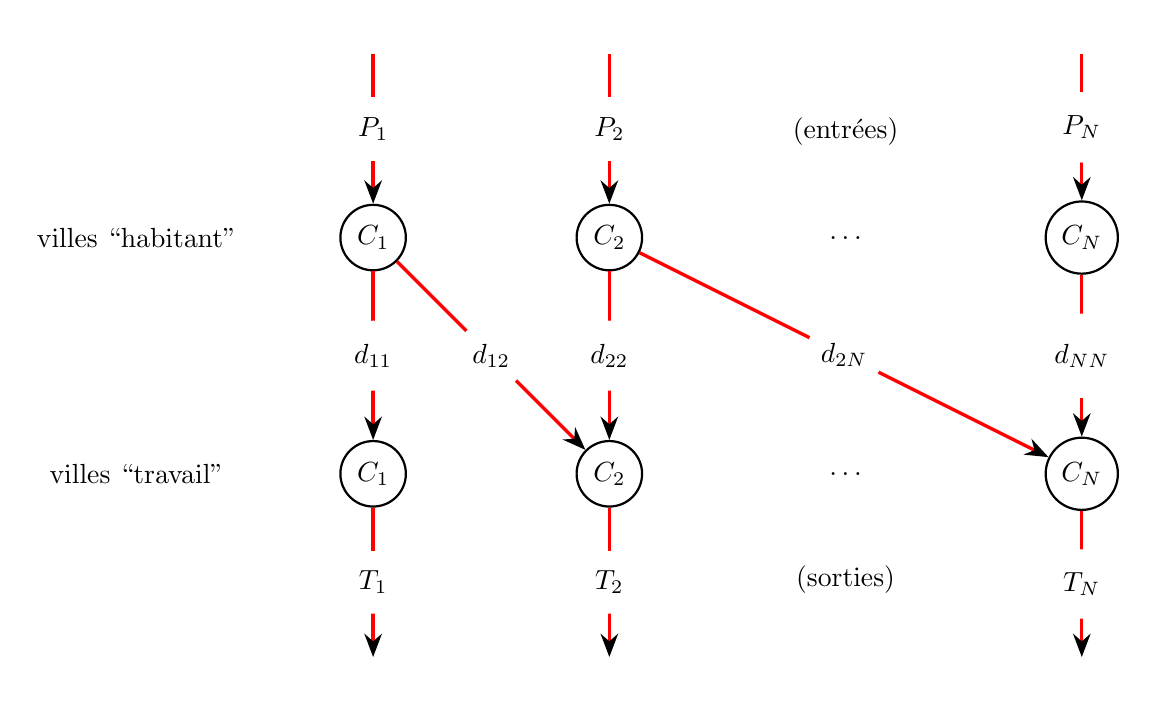
\begin{tikzpicture}
          % Villes habitant
          \begin{scope}[every node/.style={circle,thick,draw}]
              \node (C11) at (0,0) {$C_1$};
              \node (C12) at (0,-3) {$C_1$};
              \node (C21) at (3,0) {$C_2$};
              \node (C22) at (3,-3) {$C_2$};
              \node (CN1) at (9,0) {$C_N$};
              \node (CN2) at (9,-3) {$C_N$};
          \end{scope}

          % Explication
          \node [rectangle] (hab) at (-3,0) {villes ``habitant''};
          \node [rectangle] (trav) at (-3,-3) {villes ``travail''};

          % Dots
          \node [dotnode] (dots1) at (6,0) {$\dots$};
          \node [dotnode] (dots2) at (6,-3) {$\dots$};

          % Valeurs initiales
          \node [dotnode] (P1) at (0,2.5) {};
          \node [dotnode] (P2) at (3,2.5) {};
          \node [dotnode] (Pdots) at (6,2.5) {};
          \path [->] (Pdots) edge [noedge] node [rectangle] {(entrées)} (dots1);
          \node [dotnode] (PN) at (9,2.5) {};

          % Valeurs de sortie
          \node [dotnode] (T1) at (0,-5.5) {};
          \node [dotnode] (T2) at (3,-5.5) {};
          \node [dotnode] (Tdots) at (6,-5.5) {};
          \path [->] (dots2) edge [noedge] node [rectangle] {(sorties)} (Tdots);
          \node [dotnode] (TN) at (9,-5.5) {};

          % Arêtes
          \begin{scope}[>={Stealth[black]},
                        every node/.style={fill=white,circle},
                        every edge/.style={draw=red,very thick}]
              \path [->] (P1) edge node {$P_{1}$} (C11);
              \path [->] (P2) edge node {$P_{2}$} (C21);
              \path [->] (PN) edge node {$P_{N}$} (CN1);
              \path [->] (C12) edge node {$T_{1}$} (T1);
              \path [->] (C22) edge node {$T_{2}$} (T2);
              \path [->] (CN2) edge node {$T_{N}$} (TN);
              \path [->] (C11) edge node {$d_{11}$} (C12);
              \path [->] (C11) edge node {$d_{12}$} (C22);
              \path [->] (C21) edge node {$d_{22}$} (C22);
              \path [->] (C21) edge node {$d_{2N}$} (CN2);
              \path [->] (CN1) edge node {$d_{NN}$} (CN2);
          \end{scope}
          \end{tikzpicture}
     \end{center}

     Les $d_{ij}$ sont les coûts unitaires.

     Par le théorème vu au cours, il existe une solution entière à la relaxation
     continue si les données $P_i$, $T_i$ sont entières, ce qui est bien le cas,
     car on n'a pas de contraintes de capacité ici.

     \item Comparons $f_{ij}$ (avant) et $x_{ij}$ (après) : le nombre de
     déménagements causés par la réorganisation est égal à
     $\abs{f_{ij} - x_{ij}}$.

     On en tire donc les contraintes suivantes :

     \begin{enumerate}[label=(\roman*)]
          \item pour le premier cas, on a la contrainte

          \begin{align*}
               \phantom{;} \sum\limits_{i = 1}^{N} \sum\limits_{j = 1}^{N} \abs{f_{ij} - x_{ij}} \le p \left(\sum\limits_{i = 1}^{N} P_i \right);
          \end{align*}

          \item pour le second cas, on a la contrainte

          \begin{align*}
               \phantom{.} \sum\limits_{j = 1}^{N} \abs{f_{ij} - x_{ij}} \le v P_i && \forall i \in \{1, 2, \dots, N\}.
          \end{align*}
     \end{enumerate}

     Pour rendre le modèle linéaire, on ajoute $-t_{ij} \le f_{ij} - x{ij} \le
     t_{ij}$ et on remplace $\abs{f_{ij} - x_{ij}}$ par $t_{ij}$.

     Le problème original, moins contraint, a la plus petite distance. De même,
     $d(p = 0.5) \ge d(p = 0.75) \ge d(p = 1) = \textnormal{original}$ et
     $d(v = 0.25) \ge d(v = 0.5)$.

     Enfin, la contrainte \ref{i} est une relaxation de la contrainte \ref{ii},
     d'où $d(p = 0.5) \le d(v = 0.5)$.

     Au final, on a

     \begin{align*}
          \phantom{.} d(\textnormal{original}) \le d(p = 0.75) \le d(p = 0.5) \le d(v = 0.5) \le d(v = 0.25).
     \end{align*}
     \end{enumerate}
\end{solution}

\section{Analyse de tableau optimal}

On considère le problème d’optimisation linéaire

\begin{equation*}
\setlength\arraycolsep{1.5pt}
  \begin{array}{c@{\quad} r c r c r}
    \max\limits_{x_i} &     x_1 & + &    x_2 &     &               \\
    \mathrm{s.t.}     &   5 x_1 & + &  3 x_2 & \le & 10\phantom{.} \\
                      &   4 x_1 & + &    x_2 & \le &  5\phantom{.} \\
                      &     x_1 & + &  2 x_2 & \le &  8\phantom{.} \\
                      &     x_1 &   &        & \ge &  0\phantom{.} \\
                      &         &   &    x_2 & \ge &  0.
  \end{array}
\end{equation*}

\begin{enumerate}[label=(\alph*)]
     \item Formulez ce problème sous forme standard. Précisez à quelles base et
     solution admissible de base correspondent le tableau simplexe initial à
     gauche ci-dessous.

\begin{equation*}
\begin{array}{c c c c c | c}
     -1\phantom{-} & -1\phantom{-} & 0 & 0 & 0 & z\\
     \hline
     5  & 3  & 1 & 0 & 0 & 10\\
     4  & 1  & 0 & 1 & 0 &  5\\
     1  & 2  & 0 & 0 & 1 &  8\\
\end{array}
\qquad \to \qquad
\begin{array}{c c c c c | c}
     \frac{2}{3}  & 0 & \frac{1}{3}  & 0 & 0 & z + \frac{10}{3}\\
     \hline
     \frac{5}{3}  & 1 & \frac{1}{3}  & 0 & 0 &     \frac{10}{3}\\
     \frac{7}{3}  & 0 & -\frac{1}{3}\phantom{-} & 1 & 0 &      \frac{5}{3}\\
     -\frac{7}{3}\phantom{-} & 0 & -\frac{2}{3}\phantom{-} & 0 & 1 &      \frac{4}{3}\\
\end{array}
\end{equation*}

     \item L’application de l’algorithme du simplexe conduit au tableau à
     droite ci-dessus.

     \begin{enumerate}[label=(\roman*)]
          \item Quelle est la base de ce tableau ? Pourquoi ce tableau est-il
          optimal ? Quelle est la solution optimale ? Quelle est la valeur
          optimale ?

          \item Que valent\footnote{Il est possible de répondre sans calcul.}
          la matrice de base optimale $B$ et son inverse $B^{-1}$ ?

          \item Que valent les variables optimales duales $y$ ? De combien
          augmenterait l’objectif si le membre de droite de la première
          contrainte passait à $10 + \varepsilon$, pour $\varepsilon > 0$
          suffisamment petit ?

          \textit{Bonus} : Quelle est la valeur maximale d’$\varepsilon$ pour
          laquelle la base actuelle reste optimale ?
     \end{enumerate}
\end{enumerate}

\begin{solution}
     \textit{Note} : cette solution s'inspire grandement de la solution
     proposée par les enseignants.\\


     \begin{enumerate}[label=(\alph*)]
          \item Sous forme standard, ce problème devient
          \begin{equation*}
          \setlength\arraycolsep{1.5pt}
            \begin{array}{c@{\quad} r c r c r c r c r c r@{\qquad} l}
              \min\limits_{x_i} &    -x_1 & - &    x_2 &&&&&      &              &\\
              \mathrm{s.t.}     &   5 x_1 & + &  3 x_2 & + & s_1 &&&&& = & 10&\\
                                &   4 x_1 & + &    x_2 &&& + & s_2 &&& = &  5&\\
                                &     x_1 & + &  2 x_2 &&&&& + & s_3 & = &  8 &\\
                                &         &   &     x_i&&&&&&& \ge &  0& \forall i \in \{1, 2\}\\
                                &         &   &    &&&&&&s_i& \ge &  0 & \forall i \in \{1, 2, 3\}.
            \end{array}
          \end{equation*}

          $(x_1, x_2) = (0, 0)$ (et donc $(s_1, s_2, s_3) = (10, 5, 8)$) est
          une solution admissible de base, correspondant à la base $\{s_1, s_2,
          s_3\}$ et donne le tableau de gauche.

          \item Voici une analyse du tableau résolu.

          \begin{enumerate}[label=(\roman*)]
               \item Base $\{x_2, s_2,s_3\}$ : optimale car les coûts réduits
               sont positifs ou nuls.

               Solution optimale avec $x_1 = s_1 = 0$ (hors base) et
               $(x_2, s_2, s_3) = \left(\frac{10}{3}, \frac{5}{3}, \frac{4}{3}\right)$ (tableau).

               Valeur optimale :  $\zopt = -\frac{10}{3}$ (tableau). Pour le
               problème de maximisation, $\zopt = \frac{10}{3}$.

               \item
               \begin{align*}
                    \phantom{.} B &= \textnormal{colonnes de } x_2, s_2, s_3 \\
                    &= \begin{pmatrix}
                    3 & 0 & 0\\
                    1 & 1 & 0\\
                    2 & 0 & 1
               \end{pmatrix}.
               \end{align*}

               Si le tableau initial est $\irow{\cdots & B & \cdots}$, le
               tableau final est $\irow{\cdots & I & \cdots}$ (où $I$ est la
               matrice identité). Il s'obtient donc par multiplication par
               $B^{-1}$. Comme le tableau de départ était aussi $\irow{\cdots &
               I}$, le tableau final est $\irow{\cdots & B^{-1}}$, d'où

               \begin{align*}
                    \phantom{.} B^{-1} = \begin{pmatrix}
                    \frac{1}{3} & 0 & 0\\
                    -\frac{1}{3} & 1 & 0\\
                    -\frac{2}{3} & 0 & 1
               \end{pmatrix}.
               \end{align*}

               Il est bien sûr également possible d'inverser simplement $B$.

               \item On sait que $y = c_B B^{-1}$. Ici, $c_B = \irow{-1 & 0 &
               0}$ d'où $y = \irow{-\frac{1}{3} & 0 & 0}$.

               On sait aussi qu'ajouter $\Delta b$ aux contraintes ajoute
               $y^\textnormal{T} \Delta b$ à la valeur optimale (analyse de
               sensibilité via variables duales); ici on aura donc un ajout de
               $-\frac{\varepsilon}{3}$ pour le $\min$, soit encore une
               augmentation de $\frac{\varepsilon}{3}$ pour le $\max$.
          \end{enumerate}
     \end{enumerate}
\end{solution}

\section{Un investissement optimal}

Vous disposez d’un budget $B > 0$ à répartir intégralement entre trois
investissements. Après un an, chacun de ces trois investissements vous
rapportera, en fonction d'un montant investi positif $m \ge 0$, le bénéfice
$r_i(m)$ suivant :

\begin{align*}
     \phantom{.} r_1(m) = 2m \qquad \qquad r_2(m) = \ln(1 + 6m) \qquad \qquad r_3(m) = \sqrt{1 + 4m} - 1.
\end{align*}

Comment répartir votre budget entre ces trois investissements de façon
optimale, c’est-à-dire en maximisant la somme des trois bénéfices ?

\begin{enumerate}[label=(\alph*)]
          \item Formulez ce problème d’optimisation comme un problème de
          \textit{minimisation}. Est-il convexe ? Admet-il nécessairement une
          solution optimale ? (\textit{justifiez}).

          \item Écrivez les conditions d’optimalité KKT \textit{complètes} relatives à ce problème d’optimisation. La condition ILGCA est-elle satisfaite partout ? Ces conditions KKT sont-elles nécessaires ? Sont-elles suffisantes ? (\textit{justifiez})

          \item Démontrez à l’aide des conditions KKT qu’une répartition
          optimale ne peut pas faire appel au troisième investissement, quel
          que soit le budget $B$.

          \item Résolvez les conditions KKT (votre réponse dépendra de la valeur du budget $B$), puis identifiez (\textit{en justifiant}) la ou les solutions optimales au problème posé.
\end{enumerate}

\begin{solution}
     \textit{Note} : cette solution s'inspire grandement de la solution
     proposée par les enseignants.\\


     \begin{enumerate}[label=(\alph*)]
          \item La formulation du problème comme un problème de minimisation est
          la suivante :

          \begin{equation*}
          \setlength\arraycolsep{1.5pt}
            \begin{array}{c@{\quad} r c r c r c r c r@{\qquad} l}
              \min\limits_{m_i} & -2m_1 & - & \ln(1 + 6m_2) & + & 1 & - & \sqrt{1 + 4m_3} && \\
              \mathrm{s.t.} & m_1 & + & m_2 & + &&& m_3 & = & B \\
                                &&&&&&& m_i & \ge & 0 & \forall i \in \{1, 2, 3\}.
            \end{array}
          \end{equation*}

          Convexe car :

          \begin{enumerate}[label=\protect\circled{\arabic*}]
               \item \strong{Objectif convexe.}

               \subitem $-2m_1$ est convexe car c'est une fonction linéaire.
               \subitem $-\ln(1+6m_2)$ et $-\sqrt{1 + 4m_3}$ sont convexes car
               $-\ln(\cdot)$ et $-\sqrt{\cdot}$ sont des fonctions convexes, ou
               bien par calcul de la dérivée seconde de $f(m)$, $f''(m)$.

               Comme la somme conserve la convexité, la fonction objectif est
               donc convexe.

               \item \strong{Domaine convexe.}

               Le domaine est borné par des fonctions linéaires et est donc un
               polyèdre convexe.

               \item \strong{Minimisation.}

               Le problème est un problème de minimisation.
          \end{enumerate}

          Comme l'objectif est continu, et que le domaine est compact (fermé et
          borné), par le théorème des bornes atteintes le problème possède un
          minimum global.

          \item Les contraintes KKT pour ce problème sont

          \begin{align*}
               \begin{pmatrix}
                    -2\\
                    -\frac{6}{1+6m_2}\\
                    -\frac{2}{\sqrt{1+4m_3}}
               \end{pmatrix} = \begin{pmatrix}
               \lambda\\
               \lambda\\
               \lambda
          \end{pmatrix} +
          \begin{pmatrix}
               \mu_1\\
               \mu_2\\
               \mu_3
          \end{pmatrix}
          \end{align*}

          avec $\lambda$ quelconque et

          \begin{alignat*}{2}
               &\mu_i &&\ge 0 \qquad \forall i \in \{1, 2, 3\}\\
               &\mu_i m_i &&= 0 \qquad \forall i \in \{1, 2, 3\}.
          \end{alignat*}

          Les quatre contraintes sont

          \begin{align*}
               c_1(x) &\colon m_1 + m_2 + m_3 - B = 0\\
               c_2(x) &\colon m_1 \ge 0\\
               c_3(x) &\colon m_2 \ge 0\\
               c_4(x) &\colon m_3 \ge 0.
          \end{align*}

          Les gradients des contraintes sont

          \begin{align*}
               \phantom{.} \grad c_1(x) = \begin{pmatrix} 1 \\ 1 \\ 1 \end{pmatrix}; \qquad
               \grad c_2(x) = \begin{pmatrix} 1 \\ 0 \\ 0 \end{pmatrix}; \qquad
               \grad c_3(x) = \begin{pmatrix} 0 \\ 1 \\ 0 \end{pmatrix}; \qquad
               \grad c_4(x) = \begin{pmatrix} 0 \\ 0 \\ 1 \end{pmatrix}.
          \end{align*}

          Pour une dépendance, il faudrait impliquer les 4 contraintes, mais
          elles ne peuvent jamais être toutes actives (si les 3 dernières le
          sont, $\sum_{i = 1}^{3} m_i = 0 \ne B > 0$ et la première ne l'est
          donc pas).

          Comme l'ILGCA est satisfaite partout, les conditions KKT sont
          nécessaires. Elles sont également suffisantes car le problème est
          convexe.

          \item

          \begin{proof}

               Si on utilise $m_3$, c'est-à-dire $m_3 > 0$, on a $\mu_3 = 0$,
          d'où $\lambda = -\frac{2}{\sqrt{1 + 4m_3}}$.

          Cependant, la première équation donne $-2 = \lambda + \mu_1$ et $\mu_1
          \ge 0$, d'où $\lambda \le -2$.

          On déduit donc que $-\frac{2}{\sqrt{1+4m_3}} \le -2 \iff
          \sqrt{1+4m_3} \le 1 \iff m_3 \le 0 \implies m_3 > 0$.
          \end{proof}

          \item Il reste à résoudre (en sachant que $m_3 = 0$)

          \begin{align*}
               \phantom{.} \begin{pmatrix}
                    -2 \\
                    -\frac{6}{1+6m_2} \\
                    -2
               \end{pmatrix} = \begin{pmatrix}
                    \lambda + \mu_1 \\
                    \lambda + \mu_2 \\
                    \lambda + \mu_3
               \end{pmatrix}.
          \end{align*}

          On distingue quatre cas.

          \begin{enumerate}[label=\protect\fbox{\arabic*}]
               \item $\boxed{m_1 = 0 \qquad m_2 = 0}$

               C'est impossible car ($B > 0$).

               \item $\boxed{m_1 \ne 0 \qquad m_2 = 0}$

               Cela implique que $m_1 = B$, $\mu_1 = 0$.

               On déduit que

               \begin{align*}
                    \phantom{.} \begin{pmatrix}
                         -2 \\
                         -6
                    \end{pmatrix} = \begin{pmatrix}
                         \lambda \\
                         \lambda + \mu_2.
                    \end{pmatrix}.
               \end{align*}

               Cela impliquerait que $\mu_2 = -4$ ce qui est impossible.

               \item $\boxed{m_1 = 0 \qquad m_2 \ne 0}$

               Cela implique que $m_2 = B$, $\mu_2 = 0$.

               On déduit que

               \begin{align*}
                    \phantom{.} \begin{pmatrix}
                         -2 \\
                         -\frac{6}{1+6B}
                    \end{pmatrix} = \begin{pmatrix}
                         \lambda + \mu_1 \\
                         \lambda.
                    \end{pmatrix}.
               \end{align*}

               On trouve donc $\mu_1 = -2 + \frac{6}{1+6B}$. On sait que $\mu_1
               \ge 0 \iff \frac{6}{1+6B} \ge 2 \iff 3 \ge 1+6B \iff B \le
               \frac{1}{3}$.

               Dans ce cas-ci on trouve donc une solution:

               \begin{align*}
                    (m_1, m_2, m_3) = (0, B, 0) \textnormal{ si } B \le
                    \frac{1}{3}\textnormal{, impossible sinon.}
               \end{align*}

               \item $\boxed{m_1 \ne 0 \qquad m_2 \ne 0}$

               On a donc $\mu_1 = \mu_2 = 0$

               On déduit que

               \begin{align*}
                    \phantom{.} \begin{pmatrix}
                         -2 \\
                         -\frac{6}{1+6m_2}
                    \end{pmatrix} = \begin{pmatrix}
                         \lambda\\
                         \lambda.
                    \end{pmatrix}.
               \end{align*}

               On a alors $-\frac{6}{1+6m_2} = -2 \iff m_2 = \frac{1}{3}$ et
               donc $m_1 = B - \frac{1}{3}$, possible uniquement si $B \ge
               \frac{1}{3}$.

               Dans ce cas-ci on trouve donc une solution:

               \begin{align*}
                    (m_1, m_2, m_3) = \left(B-\frac{1}{3}, \frac{1}{3}, 0\right) \textnormal{ si } B \ge
                    \frac{1}{3}\textnormal{, impossible sinon.}
               \end{align*}
          \end{enumerate}

          Ces solutions KKT sont les seules solutions optimales globales
          car KKT nécessaire et suffisant.
     \end{enumerate}
\end{solution}

\section{Méthodes d'optimisation non linéaire}

\textit{Justifiez} soigneusement vos réponses, par exemple à l’aide d’un
théorème vu au cours ou d’un exemple/contre-exemple.

\begin{enumerate}[label=(\alph*)]
     \item Un problème convexe sans contrainte peut-il admettre un point de
     selle (c’est-à-dire un point stationnaire qui n’est ni minimum local ni
     maximum local) ?

     \item À quelles conditions (propriétés de la fonction à minimiser,
     longueur de pas) peut-on garantir la convergence globale de la méthode de
     la plus forte pente ?

     \item Le choix d’une longueur de pas minimisant exactement la fonction
     dans la direction choisie satisfait-il nécessairement à la première
     condition de Wolfe ? À la seconde ?

     \item Par quel moyen les méthodes de quasi-Newton peuvent-elles se passer
     de l’inversion de l’approximation de la matrice hessienne à chaque
     itération ?

     \item Quelle méthode permet d’obtenir la solution optimale d’un problème
     d’optimisation quadratique convexe après un nombre fini de pas ? Quel est
     ce nombre de pas ?
\end{enumerate}

\begin{solution}
     \textit{Note} : cette solution s'inspire grandement de la solution
     proposée par les enseignants.\\


\begin{enumerate}[label=(\alph*)]
     \item Sans contraintes, un point stationnaire annule d'office $\grad f(x)$.
     Comme le problème est convexe, $\grad f(x) = 0$ implique que $x$ soit un
     minimum global, et donc jamais un point de selle.

     \item Si $f$ est bornée inférieurement, continûment différentiable, que
     son gradient soit lipschitzien ($\norm{\grad f(x) - \grad f(y)} \le L
     \norm{x - y}$), et que le pas vérifie les conditions de Wolfe, alors on a
     la convergence globale.

     \item La condition de décroissance suffisante n'est pas toujours
     satisfaite. Cependant, la condition de courbure, elle l'est.

     En effet, au minimum, $\phi'(x) = 0$, d'où

     \begin{center}
          $\begin{cases} \phi'(x) \ge c_2 \phi'(0) \\ \abs{\phi'(x)} \le c_2 \abs{\phi'(0)}.
          \end{cases}$
     \end{center}

     \item Au lieu de maintenir à chaque itération l'approximation de la
     hessienne ($B_k$), puis de calculer

     \begin{align*}
          p_k = -B_k^{-1} \grad f(x_k),
     \end{align*}

     on met à jour directement l'approximation de l'inverse de la hessienne
     $H_k$, et on calcule, par une formule équivalente,

     \begin{align*}
          p_k = -H_k \grad f(x_k).
     \end{align*}

     \item La méthode des gradients conjugués converge en exactement $n$ pas
     (où $n$ est la dimension du problème).
\end{enumerate}

\end{solution}

\end{document}
